\documentclass[a4paper,oneside,14pt]{extarticle}

\input{auto/preamble}

\begin{document}

\makecourseworktitle
{Информатика и системы управления} % Название факультета
{Программное обеспечение ЭВМ и информационные технологии} % Название кафедры
{Разработка программного обеспечения для визуализации кинематики шестереночных механизмов} % Тема работы
{М.~А.~Жаринов/ИУ7-52Б} % Номер группы/ФИО студента (если авторов несколько, их необходимо разделить запятой)
{Н.~Н.~Мартынюк} % ФИО научного руководителя
{} % ФИО консультанта (необязательный аргумент; если консультантов несколько, их необходимо разделить запятой)


\setcounter{page}{4}

\numberlesssection{РЕФЕРАТ}
Расчётно-пояснительная записка \pageref{LastPage} страниц, \total{figure} рисунков,
\total{table} таблицы, 10 источников.

\noindent
КОМПЬЮТЕРНАЯ ГРАФИКА, КИНЕМАТИКА, ШЕСТЕРЕНОЧНЫЙ МЕХАНИЗМ, АЛГОРИТМ Z-БУФЕРА, ЗАКРАСКА ФОНГА, ПЛАНАРНЫЕ ТЕНИ, ГЕКСАГОНАЛЬНАЯ СЕТКА, C++, QT.

Объект исследования --- методы визуализации трехмерных сцен и алгоритмы моделирования кинематических связей в механизмах.

Цель работы --- разработка программного обеспечения для интерактивного конструирования и визуализации кинематики шестереночных механизмов в трехмерном пространстве.

В работе использованы методы аналитической геометрии и линейной алгебры для описания трехмерных объектов и их преобразований. Для визуализации применен метод программной растеризации с использованием алгоритма Z-буфера для удаления невидимых поверхностей. Расчет освещения выполнен с использованием модели Фонга. Для построения теней использован метод планарной проекции. Расчет кинематики базируется на представлении механизма в виде графа и алгоритме поиска в ширину (BFS).

Разработано программное обеспечение, позволяющее конструировать механизмы из зубчатых колес на гексагональной сетке, визуализировать их вращение с учетом физических связей и определять заклинивание. Реализовано корректное отображение освещения и теней.

Проведен анализ производительности системы. Установлено, что время отрисовки кадра линейно зависит от количества объектов в сцене. Программа обеспечивает интерактивную частоту кадров (около 18 FPS) при отрисовке 100 шестеренок.


\renewcommand{\contentsname}{СОДЕРЖАНИЕ}
\tableofcontents

\numberlesssection{ВВЕДЕНИЕ}

Компьютерная графика играет ключевую роль в современном инженерном проектировании, образовании и моделировании физических процессов. Визуализация сложных механических систем, в том числе зубчатых передач, позволяет наглядно демонстрировать принципы их работы, выявлять ошибки проектирования на ранних этапах и облегчает понимание кинематических связей.

Статические чертежи и двухмерные схемы не всегда способны в полной мере передать динамику взаимодействия деталей, особенно когда речь идет о сложных цепочках зацепления. Построение интерактивных трехмерных моделей, позволяющих пользователю конструировать механизмы и наблюдать за их движением в реальном времени, является актуальной задачей.

\textbf{Цель курсовой работы} --- разработка программного обеспечения для интерактивного конструирования и визуализации кинематики шестереночных механизмов в трехмерном пространстве.

Для достижения поставленной цели необходимо решить следующие \textbf{задачи}:

\begin{itemize}
	\item выполнить анализ предметной области и существующих методов визуализации трехмерных сцен и моделирования кинематических связей;
	\item выбрать алгоритмы компьютерной графики для визуализации сцены: алгоритмы удаления невидимых поверхностей, методы закраски и построения теней;
	\item разработать выбранные алгоритмы визуализации;
	\item разработать алгоритм расчета кинематики зубчатых передач для корректного вычисления скоростей и направлений вращения всех элементов цепи;
	\item спроектировать структуру программного обеспечения и реализовать его;
	\item провести тестирование программы и оценить эффективность реализованных алгоритмов.
\end{itemize}

\section{Аналитический раздел}

В данном разделе проводится анализ предметной области, формализуются объекты сцены и рассматриваются математическая модель расчета кинематики шестереночных механизмов. Также производится обзор и сравнительный анализ алгоритмов компьютерной графики для выбора наиболее подходящих алгоритмов в рамках поставленной задачи.

\subsection{Описание и формализация объектов сцены}

Сцена представляет собой трехмерное пространство, содержащее следующие типы объектов.
\begin{enumerate}
	\item Шестерни (зубчатые колеса). Являются основными динамическими объектами. Модель состоит из цилиндрического основания и зубьев, расположенных по окружности. Важными параметрами для построения являются:
	      \begin{itemize}
		      \item $R$ --- радиус делительной окружности;
		      \item $N$ --- количество зубьев (пропорционально радиусу для обеспечения зацепления);
		      \item $h$ --- толщина шестерни;
		      \item $\phi$ --- текущий угол поворота вокруг собственной оси.
	      \end{itemize}
	\item Основание (пол) --- плоскость, на которую проецируются тени объектов. На основании нанесена гексагональная сетка для удобства позиционирования.
	\item Источник света --- бесконечно удаленный объект, задается углом падения и направлением (азимутом) света.
\end{enumerate}

\subsection[Осевая система координат гексагональной сетки]{Осевая система координат гексагональной \\ сетки}
Для позиционирования объектов используется гексагональная сетка. В отличие от прямоугольной сетки, где каждый узел имеет 4 соседа, в гексагональной сетке каждый узел имеет 6 равноудаленных соседей. Эта сетка лучше подходит для размещения шестеренок, так как в данной сетке отсутствуют диагонали.
В отличие от прямоугольной сетки, где оси ортогональны, в гексагональной структуре естественным образом выделяются три оси симметрии. Для математического описания такой структуры наиболее удобна кубическая система координат $(x, y, z)$, подчиняющаяся условию $x + y + z = 0$. Однако, поскольку это условие делает одну из координат избыточной, для хранения данных и оптимизации вычислений применяется осевая система координат~\cite{redblob_hex}.

В осевой системе положение любой ячейки (шестерни) задается парой целочисленных координат $(q, r)$:
\begin{itemize}
	\item $q$ --- координата, соответствующая столбцу (направлена под углом $30^\circ$ к горизонтали);
	\item $r$ --- координата, соответствующая ряду (направлена вертикально или под углом, в зависимости от ориентации).
\end{itemize}

Третья (кубическая) координата $s$ при необходимости может быть вычислена неявно по формуле~\eqref{eq:cubic_coord}:
\begin{equation}
	s = -q - r.
	\label{eq:cubic_coord}
\end{equation}

Данная система координат позволяет выполнять операции смещения и поиска соседей с помощью простого сложения векторов, избегая сложных проверок четности строк, свойственных системам со смещением.

Для визуализации сцены необходимо преобразовать дискретные координаты сетки $(q, r)$ в непрерывные мировые координаты $(x_{world}, z_{world})$. В данной работе используется ориентация шестиугольников вершиной вверх. Преобразование осуществляется по формулам~\eqref{eq:hex_to_cartesian}.

\begin{equation}
	\label{eq:hex_to_cartesian}
	\begin{cases}
		x_{world} = S \cdot \sqrt{3} \cdot \left( q + \frac{r}{2} \right), \\
		z_{world} = S \cdot \frac{3}{2} \cdot r,
	\end{cases}
\end{equation}
где $S$ --- размер шестиугольника (радиус описанной окружности, расстояние от центра до вершины).

Обратное преобразование (нахождение ячейки $(q, r)$ по клику мыши в точку $(x, z)$) выполняется путем инверсии матрицы преобразования \eqref{eq:hex_to_cartesian} и последующего округления до ближайшего узла сетки по формуле~\eqref{eq:cartesian_to_hex}.

\begin{equation}
	\begin{cases}
		q_{float} = \frac{\frac{\sqrt{3}}{3} \cdot x_{world} - \frac{1}{3} \cdot z_{world}}{S}, \\
		r_{float} = \frac{\frac{2}{3} \cdot z_{world}}{S}.
	\end{cases}
	\label{eq:cartesian_to_hex}
\end{equation}

После получения вещественных координат $(q_{float}, r_{float})$ применяется алгоритм округления кубических координат для устранения погрешностей дискретизации и выбора корректной ячейки.

\subsection[Математическая модель кинематики механизмов]{Математическая модель кинематики \\ механизмов}

Система сцепленных шестеренок может быть представлена в виде неориентированного графа $G = (V, E)$, где $V$ --- множество шестеренок (вершин), а $E$ --- множество пар сцепленных шестеренок (ребер).

В системе присутствует один источник вращения (ведущая шестерня) с заданной угловой скоростью $\omega_{driver}$. Задача кинематического расчета сводится к определению угловых скоростей $\omega_i$ для всех остальных шестеренок.

Условие отсутствия проскальзывания в точке контакта двух шестеренок $i$ и $j$ требует равенства линейных скоростей их зубьев $v_i$ и $v_j$:
\begin{equation}
	v_i = -v_j.
\end{equation}
Знак минус обусловлен тем, что в паре внешнего зацепления шестерни вращаются в противоположных направлениях.

Связь линейной скорости $v$ и угловой скорости $\omega$ выражается формулой $v = \omega \cdot R$. Следовательно, передаточная функция для двух сцепленных шестеренок с угловыми скоростями $\omega_i$ и $\omega_j$ и радиусами $R_i$ и $R_j$ описывается уравнением~\eqref{eq:transmission_function}~\cite{artobolevsky}.
\begin{equation}
	\omega_j = -\omega_i \cdot \frac{R_i}{R_j}.
	\label{eq:transmission_function}
\end{equation}

Для распространения вращения по всей системе используется алгоритм обхода графа в ширину (BFS).
Алгоритм также должен выполнять проверку на заклинивание. Заклинивание происходит, если в графе существуют циклы, и при обходе обнаруживается, что для одной и той же шестерни приходят противоречивые требования к скорости или направлению вращения от разных соседей. Если для вершины $k$ уже вычислена скорость $\omega_k$, а новый путь от соседа $m$ требует скорости $\omega'_k$, и $|\omega_k - \omega'_k| > \varepsilon$, то система считается заклинившей.

Также для визуальной корректности необходимо учитывать фазовое смещение $\theta$, чтобы зубья одной шестерни попадали во впадины другой. Угол поворота ведомой шестерни радиусом $R_{next}$ и с количеством зубьев $N_{next}$ рассчитывается по формуле~\eqref{eq:offset}.
\begin{equation}
	\theta_{next} = \alpha \cdot (1 + \frac{R_{curr}}{R_{next}}) - \theta_{curr} \cdot \frac{R_{curr}}{R_{next}} + \pi + \frac{\pi}{N_{next}},
	\label{eq:offset}
\end{equation}
где
\begin{itemize}
	\item $\alpha$ --- угол вектора, соединяющего центры шестеренок;
	\item $\theta_{curr}$ --- фазовое смещение текущей шестерни;
	\item $\theta_{next}$ --- фазовое смещение ведомой шестерни;
	\item $R_{curr}$ --- радиус текущей шестерни.
\end{itemize}

\subsection[Математические основы построения трехмерного изображения]{Математические основы построения \\ трехмерного изображения}

Для визуализации трехмерной сцены на двумерном экране используется графический конвейер, включающий последовательность преобразований систем координат~\cite{foley}.

Любая точка $P_{local}$ из локального пространства модели преобразуется в экранные координаты $P_{screen}$ с помощью умножения на матрицы по формуле~\eqref{eq:transform}.
\begin{equation}
	P_{screen} = M_{proj} \cdot M_{view} \cdot M_{model} \cdot P_{local},
	\label{eq:transform}
\end{equation}
где
\begin{enumerate}
	\item Модельная матрица $M_{model}$ отвечает за положение, поворот и масштаб объекта в мировом пространстве. Для вращающейся шестерни эта матрица пересчитывается каждый кадр в зависимости от угла $\phi$.
	\item Видовая матрица $M_{view}$ трансформирует мировые координаты в систему координат камеры. Она определяется позицией наблюдателя, точкой, на которую он смотрит, и вектором <<вверх>>.
	\item Проекционная матрица $M_{proj}$ преобразует усеченную пирамиду видимости в куб нормализованных координат устройства. Для реалистичного отображения используется перспективная проекция, при которой удаленные объекты кажутся меньше. Элементы матрицы зависят от угла обзора и соотношения сторон экрана.
\end{enumerate}

После матричных преобразований производится перспективное деление (деление на координату $w$) и переход к экранным координатам.

\subsection[Анализ алгоритмов удаления невидимых поверхностей]{Анализ алгоритмов удаления невидимых \\ поверхностей}

При отображении трехмерных объектов на двумерном экране необходимо определить, какие части объектов видны наблюдателю, а какие скрыты другими объектами или собственными гранями. Рассмотрим основные методы решения этой задачи.

\subsubsection{Алгоритм Робертса}
Данный алгоритм работает в пространстве объекта и предназначен преимущественно для выпуклых многогранников. Алгоритм состоит из двух этапов.
\begin{enumerate}
	\item Удаление нелицевых граней. Для каждой грани вычисляется скалярное произведение вектора взгляда и внешней нормали к грани. Если результат положительный, грань <<отвернута>> от наблюдателя и отбрасывается.
	\item Сравнение каждого ребра каждого тела с остальными телами. Проверяется, экранируется ли ребро (или его часть) каким-либо другим объектом сцены.
\end{enumerate}
Алгоритм математически точен, но имеет сложность $O(N^2)$, где $N$ --- количество объектов, и плохо масштабируется для сложных сцен с невыпуклыми объектами (требует разбиения на выпуклые части)~\cite{rogers1989}.

\subsubsection{Алгоритм художника}
Алгоритм работает в пространстве объекта и изображения. Суть заключается в сортировке всех полигонов сцены по их глубине (расстоянию от наблюдателя). Отрисовка происходит в порядке от самых дальних полигонов к самым ближним. Ближние объекты перекрывают дальние в буфере кадра.
Главный недостаток алгоритма --- невозможность корректной обработки случаев циклического перекрытия (полигон A перекрывает B, B перекрывает C, C перекрывает A) и случаев взаимопересечения полигонов без их предварительного геометрического разбиения~\cite{rogers1989}.

\subsubsection{Алгоритм обратной трассировки лучей}
Метод работает в пространстве изображения. Для каждого пикселя экрана из центра проекции (глаза наблюдателя) выпускается луч. Находится ближайшая точка пересечения луча с объектами сцены. Цвет пикселя определяется свойствами объекта в точке пересечения.
Алгоритм автоматически решает проблему видимости, теней и отражений. Однако он требует больших вычислительных затрат, так как поиск пересечений должен выполняться для каждого пикселя с каждым полигоном~\cite{shikin2005}.

\subsubsection{Алгоритм, использующий Z-буфер}
Работает в пространстве изображения. Помимо буфера цвета, используется буфер глубины (Z-Buffer) той же размерности. В ячейках Z-буфера хранятся значения глубины (координаты $z$ или $1/z$) ближайшего к наблюдателю объекта, спроецированного в данный пиксель~\cite{rtr4}.
Алгоритм состоит из следующих этапов.
\begin{enumerate}
	\item Изначально Z-буфер заполняется значением бесконечности (максимальной глубины).
	\item При растеризации каждого полигона для каждого пикселя вычисляется его глубина $z_{current}$.
	\item Сравнивается $z_{current}$ со значением $z_{buffer}$, уже хранящимся в буфере.
	\item Если $z_{current} < z_{buffer}$, то пиксель ближе к наблюдателю: цвет записывается в буфер кадра, а $z_{buffer}$ обновляется значением $z_{current}$.
\end{enumerate}

\subsubsection{Сравнение алгоритмов удаления невидимых поверхностей}

Сравнение алгоритмов удаления невидимых поверхностей представлено в таблице~\ref{table:hsr}, где N --- количество объектов, n --- количество пикселей.
\begin{table}[h!]
	\caption{Сравнение алгоритмов удаления невидимых поверхностей}
	\label{table:hsr}
	\begin{tabular}{|p{3.3cm}|p{2.5cm}|p{3.2cm}|p{5cm}|}
		\hline
		Алгоритм          & Сложность      & Использование памяти & Ограничения                                \\ \hline
		Робертса          & $O(N^2)$       & $O(N)$               & Только выпуклые тела, сложность реализации \\ \hline
		Художника         & $O(N \log N)$  & $O(N)$               & Циклические перекрытия, пересечения        \\ \hline
		Трассировка лучей & $O(n \cdot N)$ & $O(N)$               & Очень низкая скорость без оптимизации      \\ \hline
		Z-буфер           & $O(n \cdot N)$ & $O(N + n)$           & Требует доп. памяти, возможен Z-fighting   \\ \hline
	\end{tabular}
\end{table}

Для выполнения работы выбран алгоритм, использующий Z-буфер. Он позволяет корректно отображать пересекающиеся объекты (ось, проходящая сквозь шестерню), прост в реализации при программной растеризации и имеет линейную зависимость времени работы от количества обрабатываемых фрагментов.

\subsection{Анализ моделей освещения и закраски}

Для придания трехмерным объектам объема и реалистичности необходимо рассчитывать взаимодействие света с поверхностью.

\subsubsection{Плоская закраска}
Вектор нормали вычисляется один раз для всего полигона (как векторное произведение двух его сторон). Освещенность рассчитывается для этого вектора, и весь полигон закрашивается одним цветом.
Метод очень быстр, но дает изображение с четко видимыми гранями (<<фасеточная>> структура). Это подходит для стилизованной графики, но плохо передает кривизну поверхностей~\cite{shikin2005}.

\subsubsection{Закраска Гуро}
Нормали задаются в вершинах полигона. Освещенность рассчитывается для каждой из трех вершин. Затем полученные цвета линейно интерполируются по поверхности треугольника в процессе растеризации.
Метод позволяет сгладить грани, но имеет существенный недостаток: зеркальные блики рассчитываются некорректно. Если блик попадает в центр полигона, а вершины освещены слабо, блик просто исчезнет~\cite{porev2002}.

\subsubsection{Закраска Фонга}
Наиболее качественный метод локального освещения. В вершинах задаются нормали. В процессе растеризации между вершинами интерполируются векторы нормалей. Освещение рассчитывается для каждого пикселя на основе интерполированной нормали.
Модель освещения Фонга включает три компоненты и считается по формуле~\eqref{eq:phong}~\cite{rogers1989}.
\begin{equation}
	I = I_{ambient} + I_{diffuse} \cdot (\vec{L} \cdot \vec{N}) + I_{specular} \cdot (\vec{R} \cdot \vec{V})^n,
	\label{eq:phong}
\end{equation}
где
\begin{itemize}
	\item $I_{ambient}$ --- фоновое освещение;
	\item $I_{diffuse}$ --- рассеянное освещение;
	\item $I_{specular}$ --- зеркальное освещение;
	\item $n$ --- показатель гладкости материала;
	\item $\vec{N}$ --- нормаль;
	\item $\vec{L}$ --- вектор на свет;
	\item $\vec{R}$ --- вектор отражения;
	\item $\vec{V}$ --- вектор на наблюдателя.
\end{itemize}
Метод дает качественные блики на криволинейных поверхностях.

\subsubsection{Сравнение методов закраски}

Пример работы методов закраски представлен на рисунке~\ref{fig:shading_example}.

\begin{figure}[h!]
	\centering
	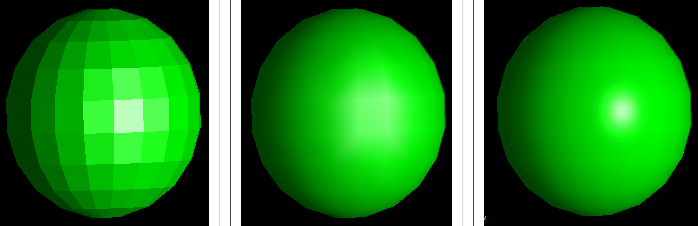
\includegraphics[width=0.8\textwidth]{img/shadingoptions.png}
	\caption{Пример работы методов закраски: слева --- плоская, в центре --- Гуро, справа --- Фонг}
	\label{fig:shading_example}
\end{figure}

Сравнение методов закраски представлено в таблице~\ref{table:shading}.

\begin{table}[h!]
	\caption{Сравнение методов закраски}
	\label{table:shading}
	\begin{tabular}{|p{3cm}|p{4cm}|p{6cm}|}
		\hline
		Метод   & Качество бликов & Вычислительные затраты \\ \hline
		Плоская & Отсутствуют     & Минимальные            \\ \hline
		Гуро    & Низкое          & Средние                \\ \hline
		Фонга   & Высокое         & Высокие                \\ \hline
	\end{tabular}
\end{table}

Для выполнения работы выбрана закраска Фонга, так как она позволяет максимально реалистично отображать блики.

\subsection{Анализ методов построения теней}

Тени являются важнейшим пространственным ориентиром, позволяющим оценить положение объектов.

\subsubsection{Теневые карты}
Алгоритм требует двух проходов рендеринга. Сначала сцена рендерится с точки зрения источника света, сохраняя только глубину. Затем, при основном рендеринге, координаты каждого пикселя преобразуются в пространство света и сравниваются с картой глубины.
Метод универсален (тени падают на любые объекты), но подвержен артефактам дискретизации (<<лесенки>> на краях теней) и сложен в реализации~\cite{porev2002}.

\subsubsection{Теневые объемы}
Геометрический метод, основанный на построении усеченных пирамид, образованных силуэтом объекта и источником света. Использует буфер трафарета для подсчета вхождений пикселя в объем тени. Дает идеально четкие края, но требует больших затрат на геометрические вычисления и сложен для моделей с большим количеством полигонов~\cite{rtr4}.

\subsubsection{Планарная проекция}
Метод применим, когда тени нужно отбрасывать только на плоскую поверхность. Геометрия объекта <<сплющивается>> на плоскость пола с помощью матрицы проекции $M_{shadow}$, которая зависит от положения источника света и уравнения плоскости. Сплющенная геометрия отрисовывается темным цветом без записи в Z-буфер.
Матрица проекции на плоскость $y=0$ для направленного света $\vec{L}$ вычисляется по формуле~\eqref{eq:shadow_matrix}.
\begin{equation}
	M_{shadow} = \begin{pmatrix}
		1 & -L_x/L_y & 0 & 0 \\
		0 & 0        & 0 & 0 \\
		0 & -L_z/L_y & 1 & 0 \\
		0 & 0        & 0 & 1
	\end{pmatrix}.
	\label{eq:shadow_matrix}
\end{equation}

\subsubsection{Сравнение методов построения теней}

Сравнение методов построения теней представлено в таблице~\ref{table:shadows}

\begin{table}[h!]
	\centering
	\caption{Сравнение методов построения теней}
	\label{table:shadows}
	\begin{tabular}{|p{3.4cm}|p{4cm}|p{2.5cm}|p{3.5cm}|}
		\hline
		Метод              & Область применения  & Качество краев & Производитель-ность         \\ \hline
		Теневые карты      & Универсальный       & Низкое         & Зависит от разрешения карты \\ \hline
		Теневые объемы     & Универсальный       & Высокое        & Низкая                      \\ \hline
		Планарная проекция & Только на плоскость & Высокое        & Высокая                     \\ \hline
	\end{tabular}
\end{table}

Для выполнения работы выбран метод планарной проекции. В задаче визуализации настольного механизма тени падают исключительно на плоскость основания (стол). Этот метод обеспечивает высокую производительность и отличное качество краев тени.

\subsection*{Вывод}

На основе проведенного анализа для реализации выбраны следующие методы:
\begin{itemize}
	\item Удаление невидимых поверхностей: Алгоритм Z-буфера, обеспечивающий корректную обработку пересекающейся геометрии.
	\item Освещение: Модель Фонга с попиксельным расчетом для качественной передачи металлических бликов.
	\item Тени: Планарная проекция на плоскость основания, как наиболее эффективный метод для данной постановки задачи.
	\item Кинематика: Графовый подход с поиском в ширину для распространения вращения и детектирования коллизий.
\end{itemize}

\section{Конструкторская часть}

В данном разделе формулируются требования к программному обеспечению, описывается общая структура программы и детально рассматриваются алгоритмы, лежащие в основе визуализации и моделирования кинематики.

\subsection{Требования к программному обеспечению}

Разрабатываемое программное обеспечение предназначено для моделирования и визуализации работы шестереночных механизмов. К программе предъявляются следующие функциональные требования:
\begin{enumerate}
	\item программа должна предоставлять графический интерфейс пользователя для взаимодействия со сценой;
	\item должна быть реализована возможность добавления шестеренок различных размеров на гексагональную сетку;
	\item должна быть предусмотрена возможность удаления установленных шестеренок;
	\item программа должна обеспечивать визуализацию трехмерной сцены, включающей пол, сетку, оси и вращающиеся шестерни;
	\item должна быть реализована возможность управления камерой (вращение вокруг центра сцены, масштабирование);
	\item программа должна моделировать кинематику механизма: передачу вращения от ведущей шестерни к ведомым с учетом передаточных чисел;
	\item должен быть реализован контроль коллизий: запрет установки шестеренок в пересекающиеся позиции;
	\item должна быть предусмотрена индикация заклинивания механизма при создании противоречивых кинематических связей;
	\item программа должна позволять управлять скоростью и направлением вращения ведущей шестерни.
\end{enumerate}

\subsection{Разработка алгоритмов}

Для реализации поставленных задач были разработаны алгоритмы визуализации и расчета физики сцены.

\subsubsection{Общая схема работы программы}

Работа программы строится на основе главного цикла обработки событий и таймера обновления кадров. Схема алгоритма работы программы представлена на рисунке \ref{img:main_algo}.

\begin{figure}[H]
	\centering
	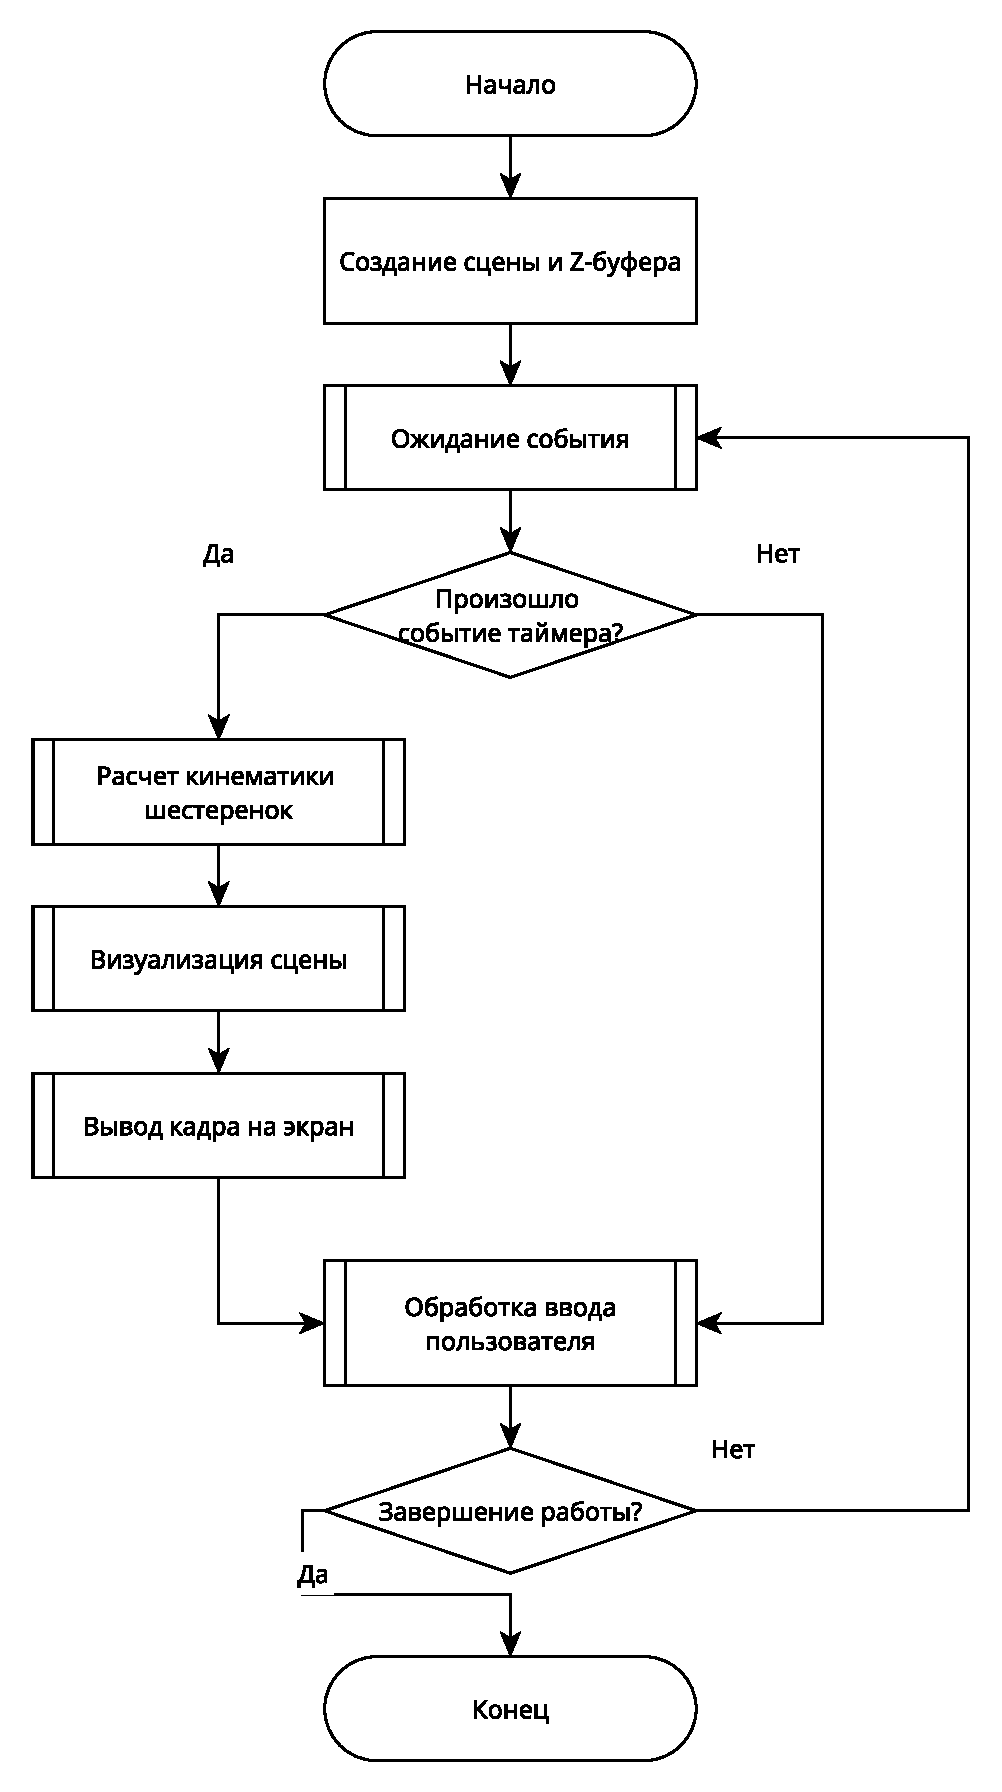
\includegraphics[width=13cm]{img/full.pdf}
	\caption{Схема алгоритма работы программы}
	\label{img:main_algo}
\end{figure}

\subsubsection{Алгоритм растеризации треугольника}

Центральным элементом графического конвейера является алгоритм растеризации треугольника с использованием Z-буфера и интерполяцией атрибутов для закраски Фонга. Схема алгоритма представлена на рисунке \ref{img:raster_algo}.

\begin{figure}[H]
	\centering
	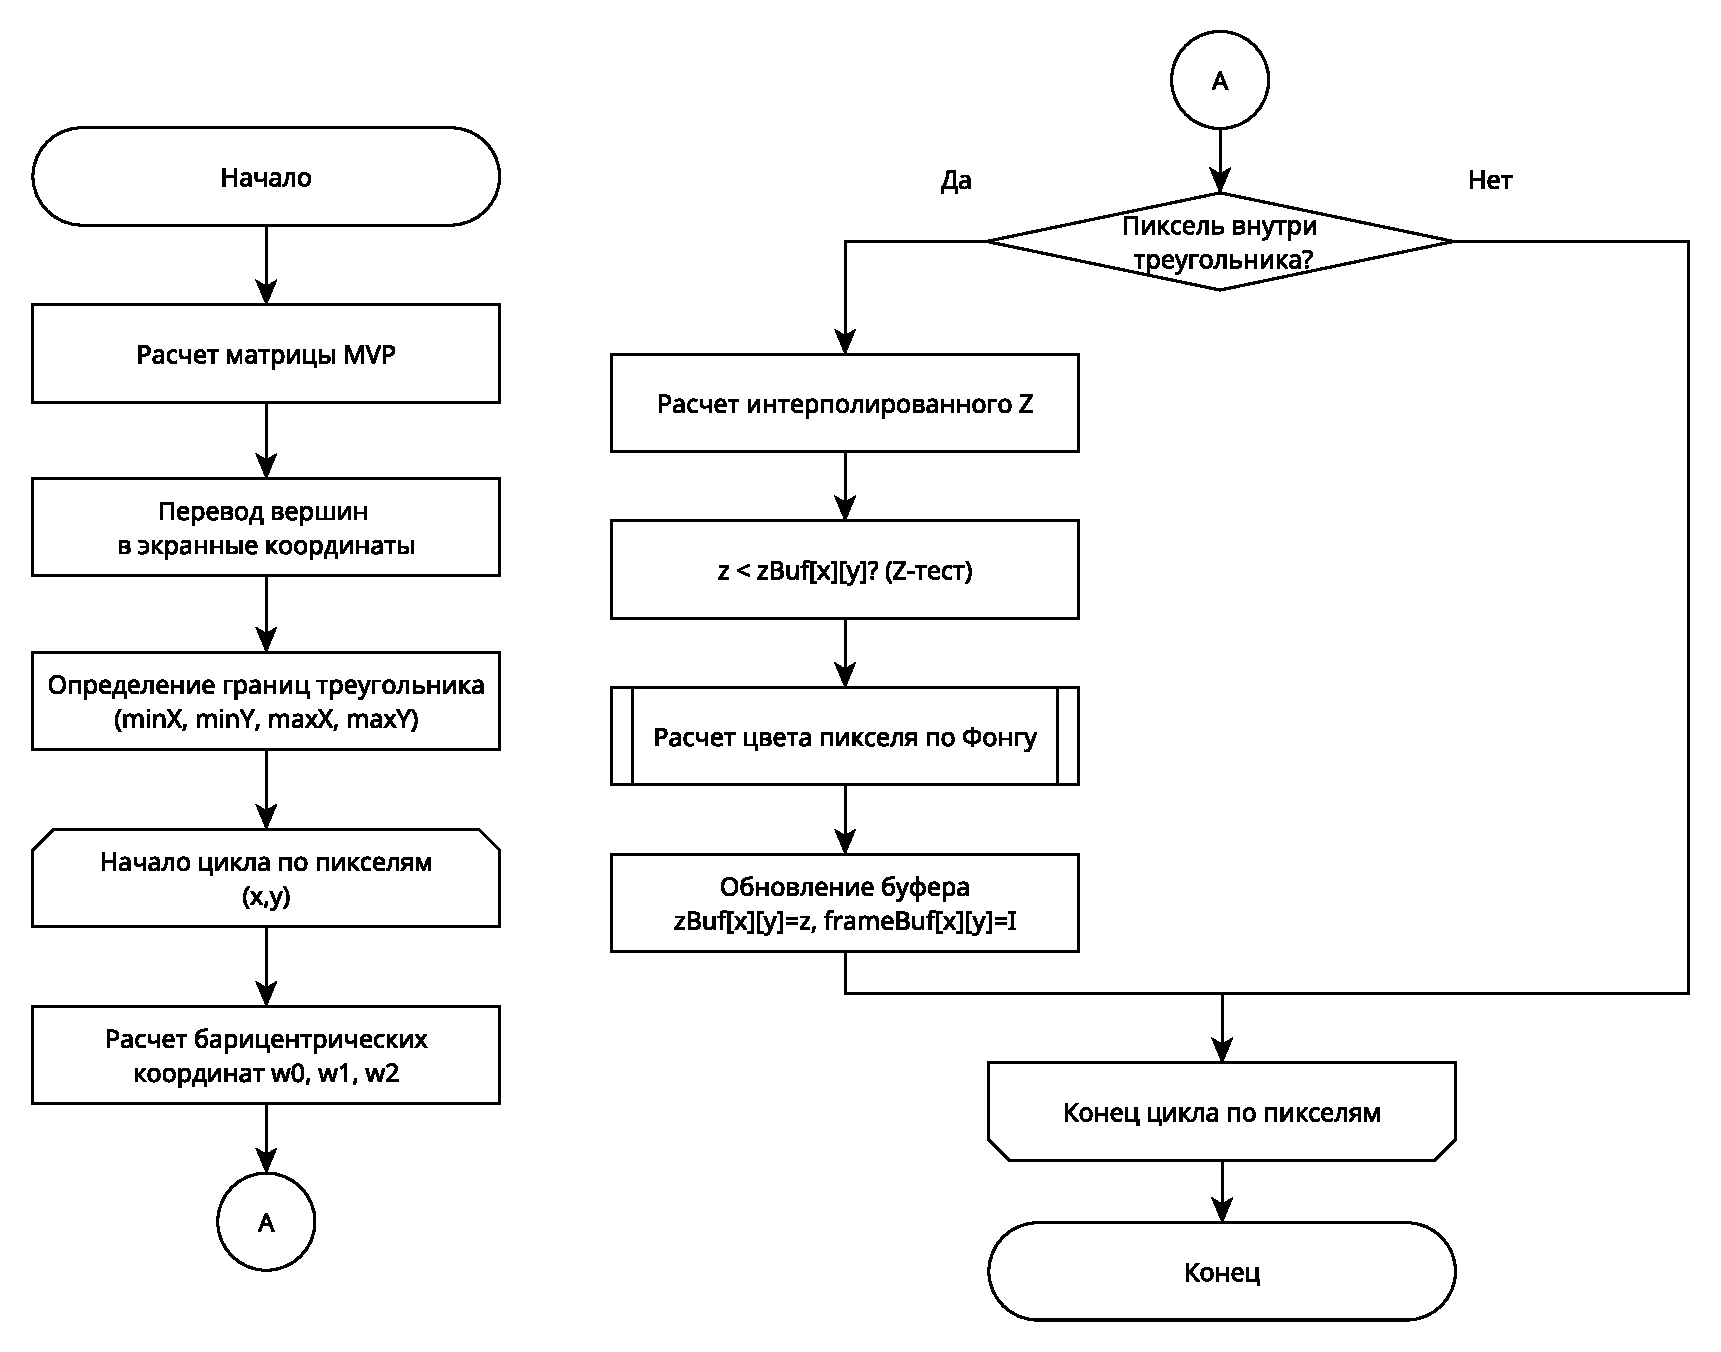
\includegraphics[width=16cm]{img/render.pdf}
	\caption{Схема алгоритма растеризации треугольника}
	\label{img:raster_algo}
\end{figure}

\subsubsection{Алгоритм расчета кинематики}

Для определения скоростей вращения всех шестеренок в механизме используется алгоритм обхода графа в ширину (BFS). Схема алгоритма представлена на рисунках~\ref{img:kinematics_algo1} и~\ref{img:kinematics_algo2}.

\begin{figure}[H]
	\centering
	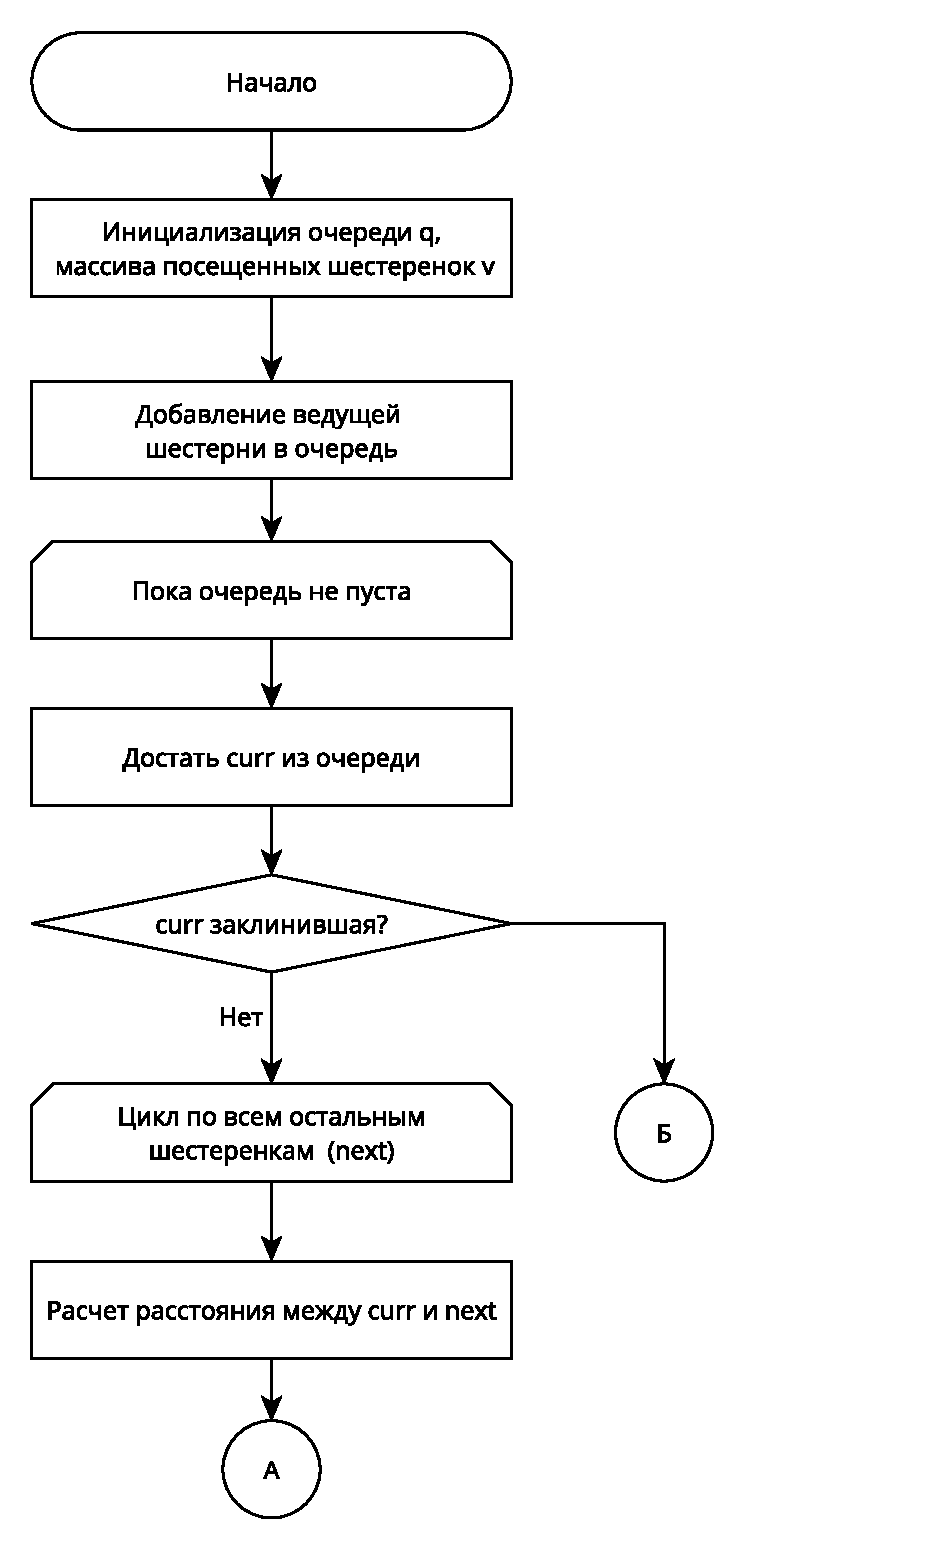
\includegraphics[width=13cm]{img/gears1.pdf}
	\caption{Схема алгоритма расчета кинематики 1}
	\label{img:kinematics_algo1}
\end{figure}
\begin{figure}[H]
	\centering
	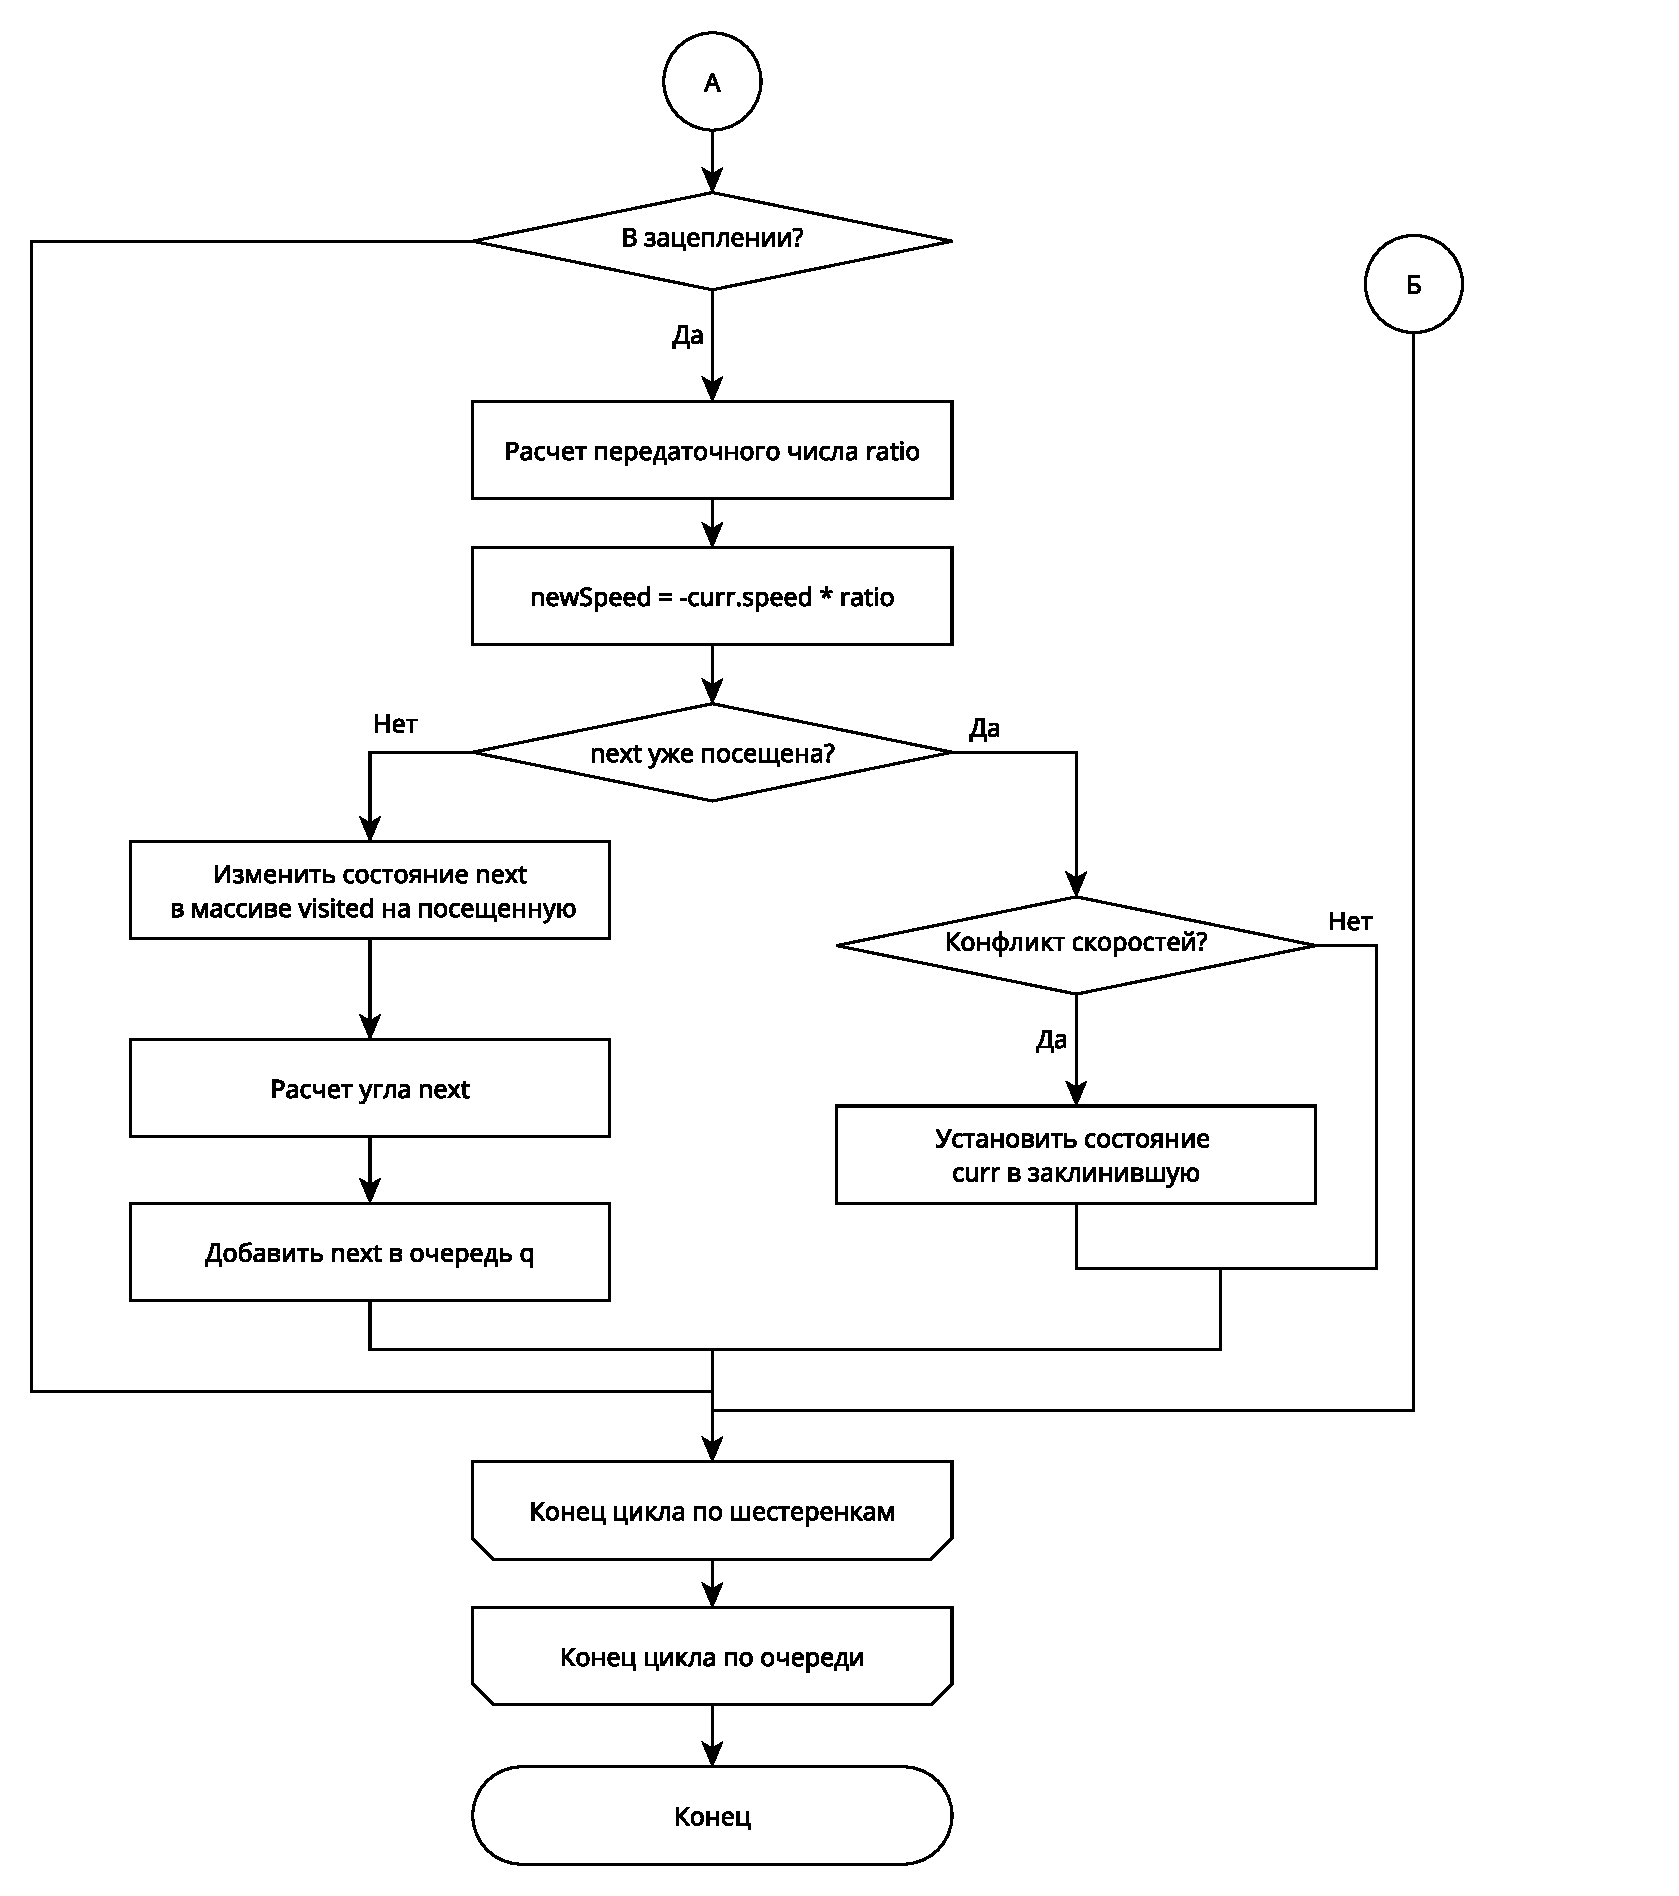
\includegraphics[width=17cm]{img/gears2.pdf}
	\caption{Схема алгоритма расчета кинематики 2}
	\label{img:kinematics_algo2}
\end{figure}


\subsection*{Вывод}

В данном разделе были сформулированы требования к программному обеспечению, включающие функциональные возможности визуализации и управления сценой. Описаны основные алгоритмы визуализации и расчета кинематики.

\section{Технологическая часть}

В данном разделе обосновывается выбор средств реализации, приводится описание структуры разработанного программного обеспечения, а также представлены листинги реализации ключевых алгоритмов визуализации и расчета кинематики.

\subsection{Выбор средств реализации}

Для разработки программы был выбран язык программирования C++~\cite{cpp_ref} (стандарт C++20). В качестве графической библиотеки и фреймворка для создания пользовательского интерфейса использована библиотека Qt~\cite{qt_doc} (версия 6). Она предоставляет:
\begin{itemize}
	\item кроссплатформенные средства создания оконного интерфейса (модуль \texttt{QtWidgets});
	\item оптимизированные математические классы (\texttt{QVector3D}, \texttt{QMatrix4x4});
	\item класс \texttt{QImage} для удобного вывода сформированного буфера кадра на экран.
\end{itemize}

Среда разработки --- Zed editor, система сборки --- qmake.

\subsection{Структура программного обеспечения}

Программа реализована с использованием принципов объектно-ориен-тированного программирования. Архитектура приложения включает следующие основные классы и структуры:

\begin{itemize}
	\item \texttt{MainWindow} — класс главного окна приложения. Отвечает за инициализацию графического интерфейса пользователя и обработку сигналов от элементов управления (кнопок, слайдеров, чекбоксов).

	\item \texttt{RenderWidget} — класс виджета для вывода трехмерной графики. Реализует цикл с использованием таймера, обрабатывает события ввода (нажатия клавиш мыши, перемещение курсора, прокрутку колеса) и управляет взаимодействием между пользователем и сценой.

	\item \texttt{Renderer} — класс, инкапсулирующий логику программного рендеринга. Содержит методы для:
	      \begin{itemize}
		      \item трансформации вершин из локального пространства в экранное;
		      \item растеризации треугольников с использованием барицентрических координат;
		      \item управления Z-буфером для удаления невидимых поверхностей;
		      \item расчета освещения по модели Фонга для каждого пикселя;
		      \item отрисовки теней методом планарной проекции.
	      \end{itemize}

	\item \texttt{Scene} — класс, описывающий состояние виртуального мира. Хранит контейнер объектов (шестеренок), параметры гексагональной сетки и геометрию статического окружения (пола). Реализует алгоритмы кинематики: поиск ведущей шестерни, распространение вращения по графу сцеплений и детектирование заклинивания механизма.

	\item \texttt{Camera} — класс виртуальной камеры. Отвечает за формирование матриц вида и проекции. Реализует управление положением наблюдателя в сферических координатах (азимут, угол места, радиус) и предоставляет функционал для генерации лучей из экранных координат в мировое пространство.

	\item \texttt{Gear} — класс, описывающий отдельную шестеренку. Содержит параметры объекта (радиус, количество зубьев, текущий угол поворота) и методы для процедурной генерации полигональной сетки (вершин и нормалей) тела шестерни и её оси вращения.

	\item \texttt{Geom.h} — заголовочный файл, содержащий вспомогательные структуры данных: \texttt{Vertex} (вершина с координатами и нормалью) и \texttt{Triangle} (набор из трех вершин и цвета).
\end{itemize}

\clearpage

Диаграмма классов представлена на рис. \ref{fig:diagram}.

\begin{figure}[H]
	\centering
	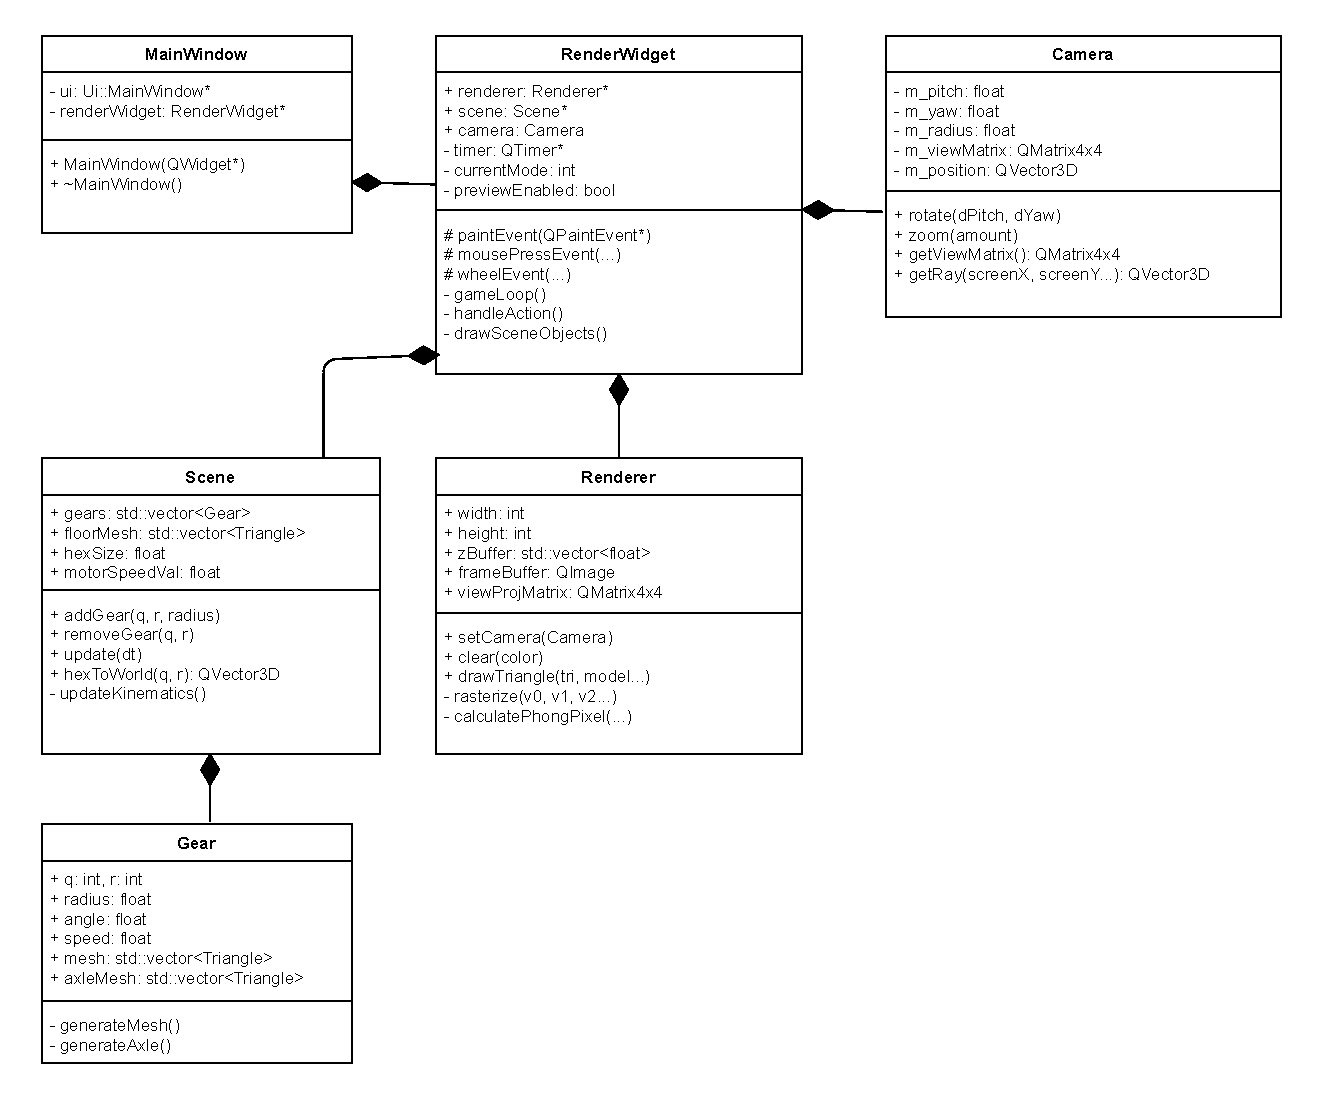
\includegraphics[width=\textwidth]{img/uml.pdf}
	\caption{Диаграмма классов}
	\label{fig:diagram}
\end{figure}

Диаграмма компонентов представлена на рис. \ref{fig:diagram_mod}.

\begin{figure}[H]
	\centering
	
\includegraphics[width=\textwidth]{img/mod.pdf}
	\caption{Диаграмма компонентов}
	\label{fig:diagram_mod}
\end{figure}

\clearpage

\subsection{Реализация алгоритмов визуализации}

Ключевым этапом визуализации является растеризация треугольников с использованием Z-буфера и интерполяцией нормалей для освещения Фонга.

В листинге \ref{lst:rasterize} приведен метод растеризации, который принимает три вершины, прошедшие вершинные преобразования, и заполняет пиксели в буфере кадра.

\begin{lstlisting}[caption={Реализация алгоритма растеризации с Z-буфером}, label={lst:rasterize}]
void Renderer::rasterize(const RasterVertex& v0, const RasterVertex& v1, const RasterVertex& v2, const RenderSettings& settings) {
    int minX = std::max(0, (int)std::min({v0.screenPos.x(), v1.screenPos.x(), ...}));
    int maxX = std::min(width - 1, (int)std::max({v0.screenPos.x(), ...}) + 1);
    int minY = std::max(0, ...}));
    int maxY = std::min(height - 1, ...}) + 1);
    float area = edgeFunction(v0, v1, v2);
    float invArea = 1.0f / area;
    for (int y = minY; y <= maxY; y++) {
        uint32_t* scanline = (uint32_t*)frameBuffer.scanLine(y);
        for (int x = minX; x <= maxX; x++) {
            float w0 = edgeFunction(v1, v2, x, y) * invArea;
            float w1 = edgeFunction(v2, v0, x, y) * invArea;
            float w2 = 1.0f - w0 - w1;
            if (w0 >= 0 && w1 >= 0 && w2 >= 0) {
                float z = w0 * v0.screenPos.z() + w1 * v1.screenPos.z() + ...;
                if (zBufferTest(x, y, z)) {
                    updateZBuffer(x, y, z);
                    if (settings.isShadow) {
                        scanline[x] = qRgb(30, 30, 30);
                    } else {
                        QVector3D normal = v0.normal * w0 + v1.normal * w1 + ...;
                        QVector3D worldPos = v0.worldPos * w0 + v1.worldPos * w1 + ...;
                        scanline[x] = calculatePhongPixel(worldPos, normal, settings);
                    }
                }
            }
        }
    }
}
\end{lstlisting}

\subsection{Реализация алгоритма кинематики}

Для расчета вращения используется алгоритм обхода графа в ширину (BFS). Метод \texttt{updateKinematics} обновляет скорости и углы поворота всех шестеренок в цепи, исходя из параметров ведущей шестерни. Реализация представлена в листинге \ref{lst:kinematics}.

\begin{lstlisting}[caption={Реализация алгоритма расчета кинематики}, label={lst:kinematics}]
void Scene::updateKinematics() {
    for (auto& g : gears) {
        if (!g.isDriver) g.speed = 0;
        else g.speed = driverSpeed;
        g.isJam = false;
    }
    std::queue<int> q;
    q.push(driverIdx);
    visited[driverIdx] = true;

    while(!q.empty()) {
        int currIdx = q.front(); q.pop();
        Gear& curr = gears[currIdx];
        if (curr.isJam) continue;
        for (size_t i = 0; i < gears.size(); i++) {
            if (isConnected(curr, gears[i])) {
                float ratio = curr.radius / gears[i].radius;
                float newSpeed = -curr.speed * ratio;
                if (visited[i]) {
                    if (std::abs(gears[i].speed - newSpeed) > EPSILON) {
                        curr.isJam = true;
                    }
                } else {
                    gears[i].speed = newSpeed;
                    visited[i] = true;
                    syncPhase(curr, gears[i]);
                    q.push((int)i);
                }
            }
        }
    }
}
\end{lstlisting}

\subsection{Интерфейс пользователя}

Графический интерфейс пользователя (GUI) разработан с использованием дизайнера форм Qt Designer и сохранен в файле \texttt{MainWindow.ui}. Интерфейс включает в себя:
\begin{enumerate}
	\item Область рендеринга: занимает большую часть окна, отображает трехмерную сцену. Поддерживает управление камерой мышью (ЛКМ — вращение, колесо — масштабирование).
	\item Панель управления: расположена слева и содержит:
	      \begin{itemize}
		      \item выбор размера добавляемой шестерни;
		      \item режим удаления объектов;
		      \item переключатель режима предпросмотра;
		      \item управление ведущей шестерней: направление (по/против часовой) и слайдер скорости.
	      \end{itemize}
\end{enumerate}

Обработка событий ввода реализована в классе \texttt{RenderWidget}. Метод \texttt{handleAction} использует класс \texttt{Camera} для построения луча из точки клика мыши и нахождения соответствующей ячейки гексагональной сетки.

Интерфейс главного окна изображен на рисунке \ref{img:main_window}.

\begin{figure}[H]
	\centering
	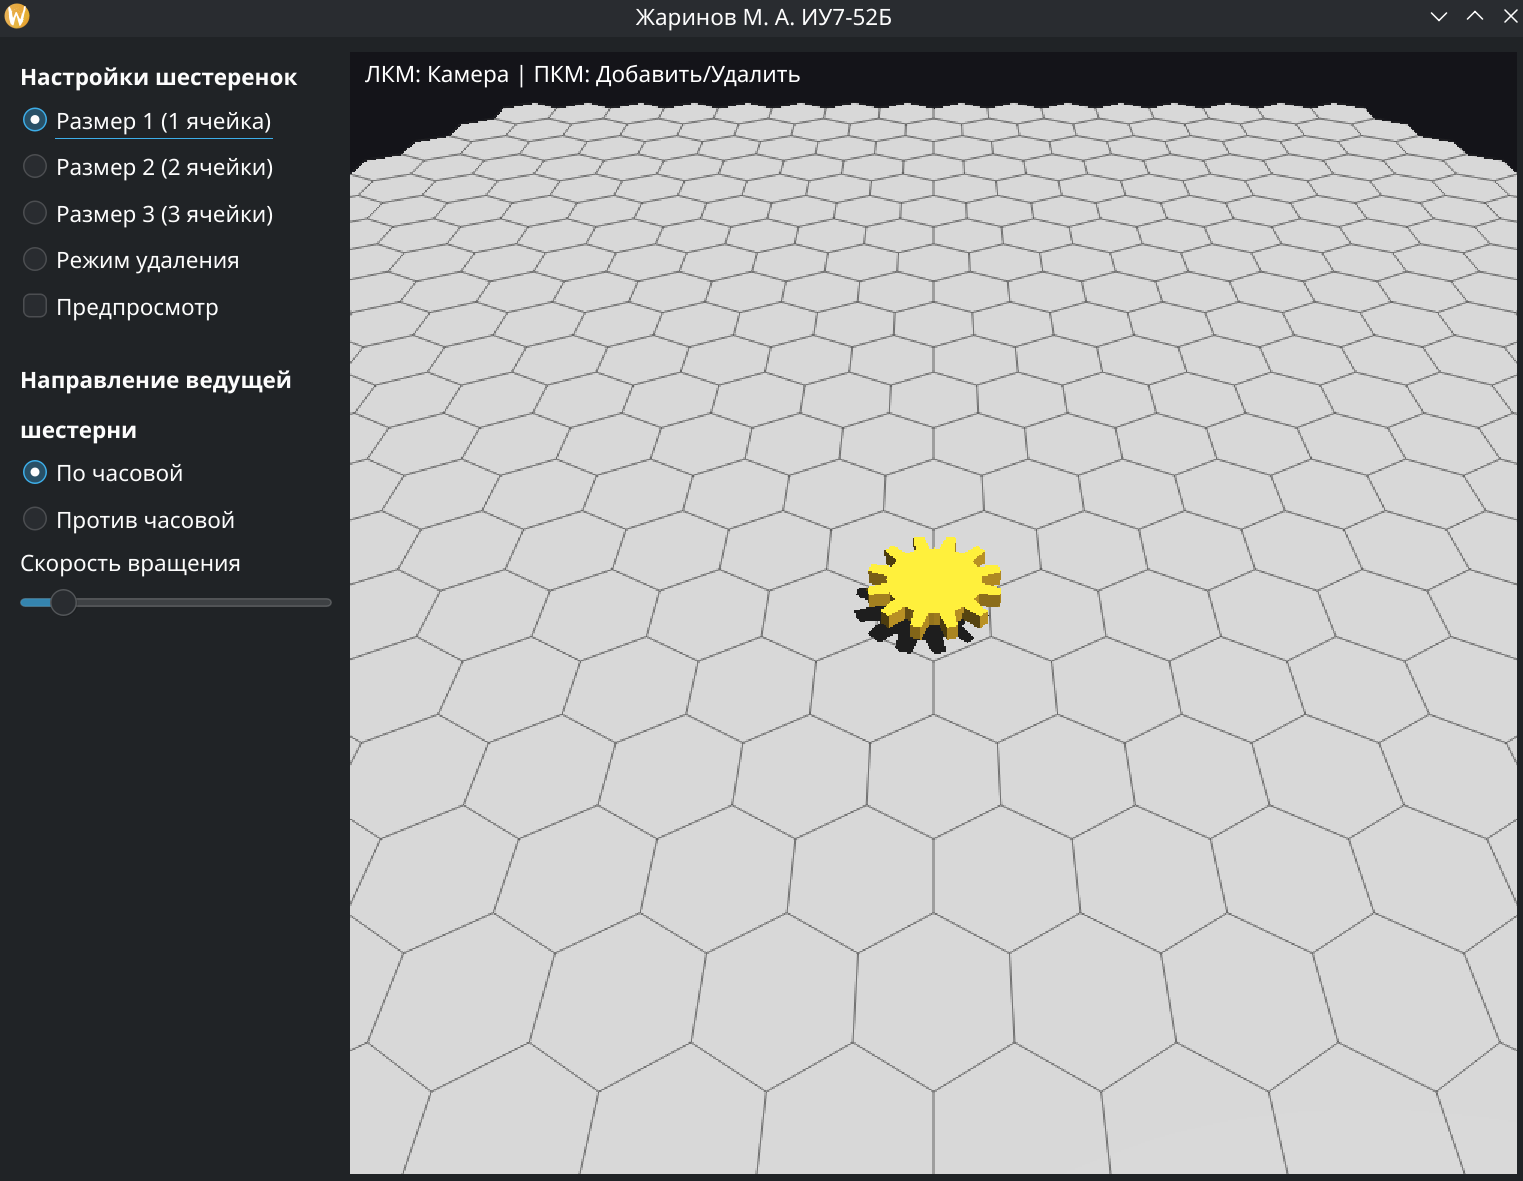
\includegraphics[width=\textwidth]{img/main_window.png}
	\caption{Главное окно программы}
	\label{img:main_window}
\end{figure}

\subsection*{Вывод}

В данном разделе описаны средства реализации и архитектура программного комплекса. Приведены реализации основных алгоритмов: растеризации треугольника с учетом Z-буфера и освещения, а также распространения кинематических связей в системе шестеренок.

\section{Исследовательская часть}

\subsection{Цель исследования}

Целью исследования является оценка производительности разработанного алгоритма программной растеризации. Необходимо установить зависимость среднего времени отрисовки одного кадра от количества геометрических объектов (шестеренок) в сцене.

\subsection{Технические характеристики}

Исследование проводилось на ноутбуке со следующими характеристиками:
\begin{itemize}
	\item операционная система --- Debian Unstable GNU/Linux с ядром версии 6.17.12;
	\item процессор --- AMD Ryzen 5 7535HS с 6 физическими ядрами и 12 логическими ядрами с максимальной тактовой частотой 4.60~ГГц~\cite{ryzen};
	\item оперативная память --- 16~Гбайт типа LPDDR5 в 4 каналах с тактовой частотой 6400~MГц.
\end{itemize}

\subsection{Алгоритм проведения исследования}

\begin{enumerate}
	\item Приложение запускается в режиме тестирования производительности.
	\item Камера фиксируется.
	\item Производится замер времени выполнения функции отрисовки кадра для количества шестеренок на сцене от 2 до 100 с шагом 2.
	\item Для каждого замера производится 100 повторений (отрисовок кадра), усредняется и сохраняется в файл.
\end{enumerate}

\subsection{Результаты исследования}

В таблице \ref{table:benchmark} приведены полученные данные.

\begin{table}[H]
	\caption{Зависимость времени рендеринга от количества объектов}
	\label{table:benchmark}
	\normalsize
	\begin{tabular}{|c|c||c|c||c|c|}
		\hline
		N, шт. & T, мс   & N, шт. & T, мс   & N, шт. & T, мс   \\ \hline
		2      & 21.3832 & 36     & 32.0729 & 70     & 44.1520 \\ \hline
		4      & 22.2666 & 38     & 32.5122 & 72     & 44.5449 \\ \hline
		6      & 22.9500 & 40     & 33.4331 & 74     & 45.1821 \\ \hline
		8      & 23.7334 & 42     & 34.4030 & 76     & 45.7830 \\ \hline
		10     & 24.3168 & 44     & 35.3910 & 78     & 45.9031 \\ \hline
		12     & 25.4002 & 46     & 35.7086 & 80     & 46.9414 \\ \hline
		14     & 25.4836 & 48     & 36.0991 & 82     & 47.0862 \\ \hline
		16     & 26.3670 & 50     & 36.8994 & 84     & 47.7650 \\ \hline
		18     & 27.0504 & 52     & 37.7999 & 86     & 48.1849 \\ \hline
		20     & 27.5338 & 54     & 37.6583 & 88     & 48.7174 \\ \hline
		22     & 28.0172 & 56     & 38.1220 & 90     & 49.0622 \\ \hline
		24     & 29.1006 & 58     & 38.9347 & 92     & 50.0099 \\ \hline
		26     & 29.3729 & 60     & 39.4367 & 94     & 51.2052 \\ \hline
		28     & 30.0054 & 62     & 40.4037 & 96     & 52.6742 \\ \hline
		30     & 30.2218 & 64     & 41.5348 & 98     & 53.9166 \\ \hline
		32     & 30.6255 & 66     & 42.3975 & 100    & 54.8800 \\ \hline
		34     & 31.1867 & 68     & 43.3006 &        &         \\ \hline
	\end{tabular}
\end{table}

На рисунке \ref{img:graph} представлен график зависимости времени кадра от количества шестеренок.

\begin{figure}[H]
	\centering
	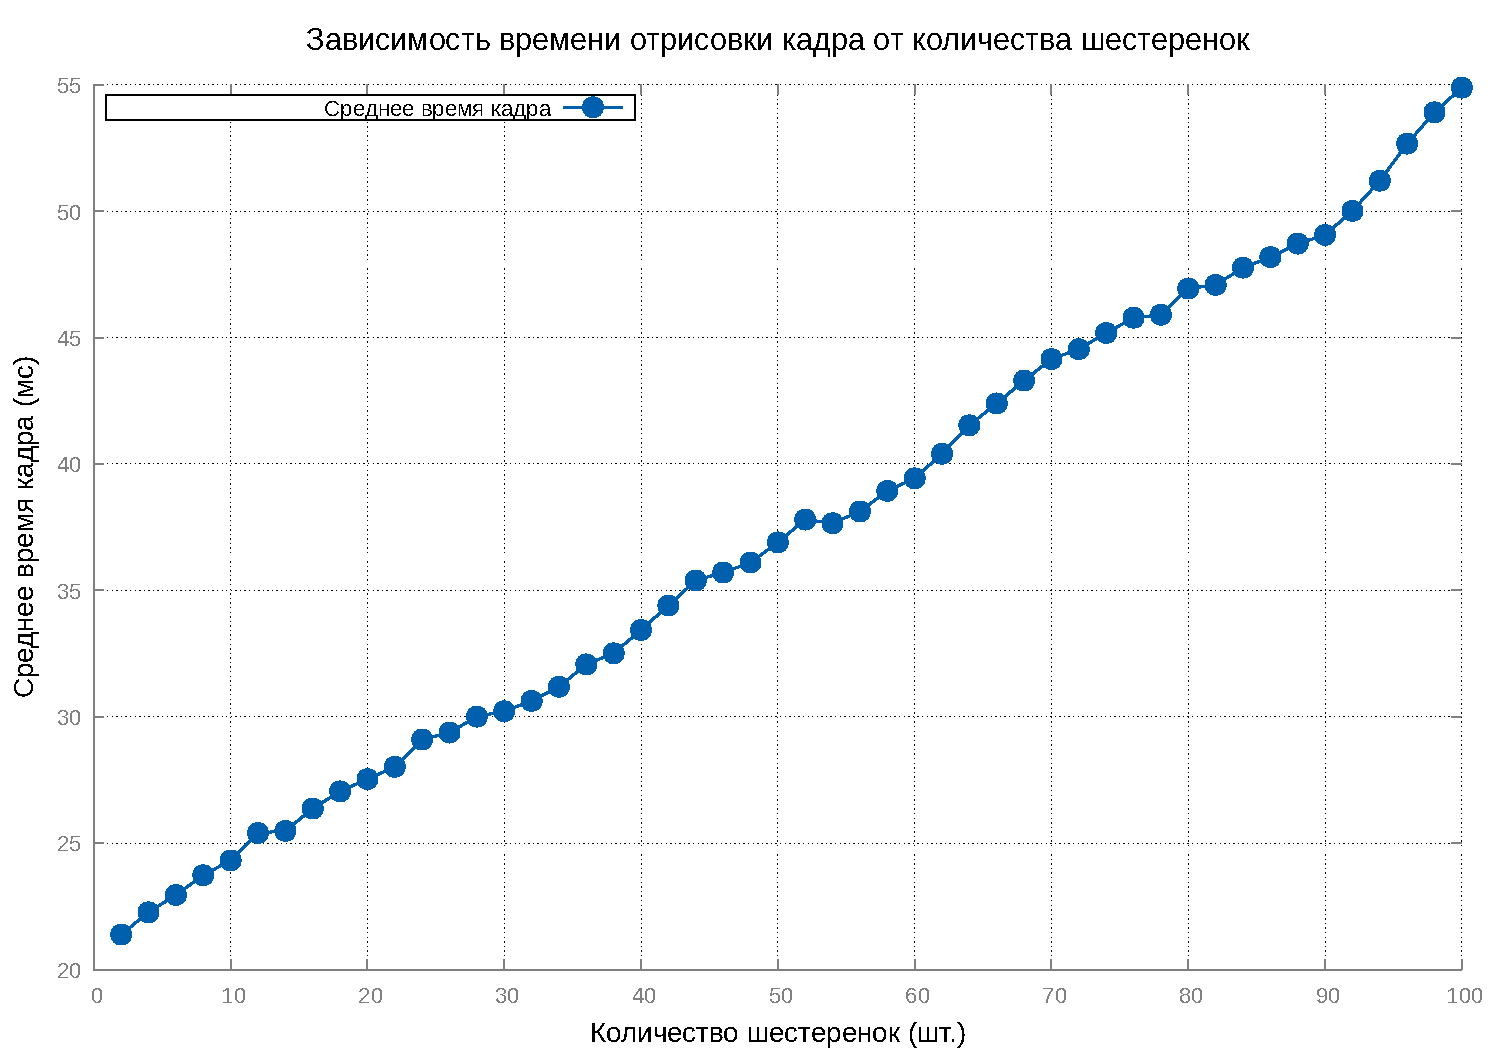
\includegraphics[width=0.9\textwidth]{img/benchmark_graph.pdf}
	\caption{График зависимости времени рендеринга от числа объектов}
	\label{img:graph}
\end{figure}

\subsection{Анализ результатов}

Зависимость времени рендеринга от количества объектов носит линейный характер. Это согласуется с теоретической оценкой сложности алгоритма растеризации и Z-буфера.

При увеличении количества объектов с 2 до 100 (рост в 50 раз), время кадра увеличилось с $\approx 21$ мс до $\approx 55$ мс (рост в 2.6 раза). Это свидетельствует о том, что значительную часть времени занимает отрисовка статического окружения и очистка буферов высокого разрешения, а добавление новой геометрии обрабатывается достаточно эффективно.

При 100 шестеренках время кадра составляет 54.8 мс, что соответствует частоте кадров $\approx 18$ FPS, что обеспечивает достаточную интерактивность приложения.

\subsection*{Вывод}

Проведенное исследование подтвердило линейную зависимость времени рендеринга от количества геометрических примитивов в сцене. Установлено, что разработанная программная реализация обеспечивает приемлемую производительность при нагрузке в 100 сложных объектов с учетом затрат на расчет теней и освещения на центральном процессоре. Полученные характеристики подтверждают эффективность выбранных алгоритмов и структур данных.

\numberlesssection{ЗАКЛЮЧЕНИЕ}

В результате выполнения курсовой работы была достигнута поставленная цель: разработано программное обеспечение для интерактивного конструирования и визуализации кинематики шестереночных механизмов в трехмерном пространстве.

В ходе работы были решены следующие задачи:
\begin{enumerate}
	\item Выполнен анализ предметной области, в ходе которого были рассмотрены математические основы построения трехмерных изображений и методы моделирования механических связей.
	\item Формализовано описание объектов сцены: определена геометрия зубчатых колес, осей и основания. Для позиционирования элементов механизма выбрана и математически описана осевая система координат гексагональной сетки, что позволило обеспечить корректное размещение сцепленных шестерен.
	\item Обоснован выбор и осуществлена программная реализация базовых алгоритмов машинной графики. Для удаления невидимых поверхностей применен алгоритм Z-буфера, обеспечивающий корректное отображение пересекающейся геометрии. Реалистичность изображения достигнута за счет использования модели освещения Фонга и алгоритма планарных теней.
	\item Разработан алгоритм расчета кинематики, основанный на представлении механизма в виде графа и его обходе в ширину. Алгоритм успешно вычисляет передаточные отношения, угловые скорости и направления вращения для всей цепи, а также детектирует ситуации механического заклинивания.
	\item Спроектирована модульная структура программного обеспечения, выделяющая слои логики (сцена, кинематика) и представления (отрисовка, интерфейс). Приложение реализовано на языке C++ (стандарт C++20) с использованием библиотеки Qt.
	\item Проведено исследование разработанного программного комплекса. Результаты показали, что время отрисовки кадра зависит линейно от количества объектов в сцене. Установлено, что разработанная программная реализация обеспечивает приемлемую производительность при нагрузке в 100 сложных объектов.
\end{enumerate}

\include{parts/07-bibliography}
\numberlesssection{ПРИЛОЖЕНИЕ А}

К расчетно-пояснительной записке курсовой работы прилагаются следующие материалы:
\begin{enumerate}
	\item презентация к курсовой работе, состоящая из 16 слайдов;
	\item USB-флеш-накопитель с исходными кодами, электронными версиями РПЗ и презентации.
\end{enumerate}


\end{document}
